% Drawing 148/01-11 -- folder 148, batch 01, archive page 17 (PDF page 18).
% Transcription: au-dessous, seconde sphère : un équateur et quatre points (un en haut, un en bas, un petit cercle à droite sur l'équateur, un groupe de quatre points à gauche). À sa droite, au milieu de la page, un petit croquis d'une sphère à quatre trous (« pantalon » à quatre jambes), la ceinture marquée en rouge.
% Kind: sphere with equator and four points; small sphere with four holes. Method 2 (schematic redraw from the facsimile). Status: ok.
% Notes: Ink. Left: a sphere outline (two strokes meeting at the upper right); a point at the top and one at the bottom of the outline; the front of the equator from the left edge of the outline to a small open circle on the right; on the left of the equator a small ring with four blots round it (the « groupe de quatre points »); the back of the equator in dashes on the left and one dash at the right; on the back above the equator a small loop with two dots and a short stroke inside (a hole or a point seen from behind; not named by the transcription). Right (figure 2): a sphere with four tubular ends, each closed by a small oval, its sides curving inwards between the ends, and two strokes across its waist, the left one heavy and dark, the right one lighter and brownish. Redrawn 2026-11-12 (issue 128). 2026-11-13, Claude Opus 5.5, issue 147, overlay check: not compiled (no TeX in the session); the TikZ was rasterised by a local interpreter and laid over the 236 ppi scan rendered at 400 dpi. Redrawn on the ink: outlines, equator and the sides of the second figure through points moved onto their ink, ovals fitted as ellipses on their ink, points on the centres of their blots; every stroke lies on its ink to within about half a unit. Changed: the second figure is no longer schematic (its sides curve inwards, its ovals are where and as large as on the page); the cluster is a ring with four blots; the small loop on the back is now drawn; the strokes across the waist are drawn in ink and brown, not red. Disagreement with the transcription: the waist of the four-holed sphere is not marked in red: the left stroke is dark ink, the right one a lighter brown (colour scan, 400 dpi).
% Coordinates: 1 unit = 1 mm = 1/100 of the crop width, y downwards as on the crop (bbox in page fractions: [0.1, 0.425, 0.48, 0.555]).
% Redrawn by Claude (claude-fable-5-2), issue #128, 2026-11-12; not checked by a human; not compiled (no TeX in the session); overlay-checked on the scan by Claude Opus 5.5, issue #147, 2026-11-13, not compiled (no TeX in the session).
% Rights: reproduces part of the work -- behind RENDER_TRANSCRIPTS, never published by itself.
\documentclass[tikz,border=3pt]{standalone}
\usepackage{amsmath,amssymb}
\usetikzlibrary{patterns,arrows.meta}
\tikzset{pencil/.style={black!45}, struck/.style={black!35}, mpt/.style={circle,draw,inner sep=1.3pt}, pt/.style={circle,fill,inner sep=0.9pt}, opt/.style={circle,draw,fill=white,inner sep=1.1pt}, Rd/.style={red!75!black}, Gn/.style={green!45!black}, Br/.style={brown!70!black}}
\begin{document}
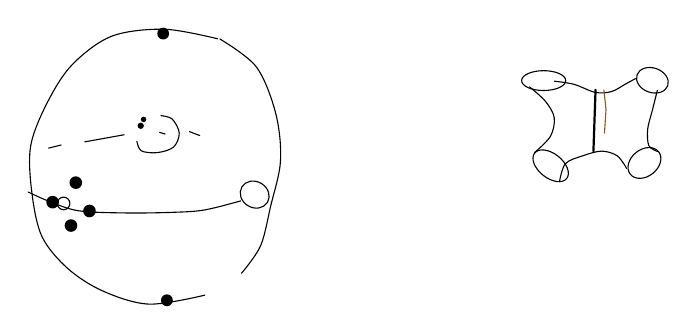
\begin{tikzpicture}[x=1mm,y=-1mm,line cap=round,line join=round,font=\small]
% first sphere: the outline (two strokes meeting at the upper right), a point at the top and one at the bottom
\draw plot[smooth, tension=0.55] coordinates {(31.67,7.51) (24.93,6.3) (18.23,7.18) (13.23,10.77) (10.1,15.5) (7.94,21.06) (8.07,26.94) (9.36,32.62) (12.66,36.7) (17.15,39.57) (23,41.21) (30.05,40.07)};
\draw plot[smooth, tension=0.55] coordinates {(31.96,7.54) (36.58,11.07) (39.05,16.98) (39.66,23) (38.4,28.8) (37.12,33.82) (34.71,37.29)};
\fill (24.76,6.85) circle [radius=0.75];
\fill (25.23,40.72) circle [radius=0.75];
% the equator: its front from the left edge to a small circle at the right; its back dashed on the left
\draw plot[smooth, tension=0.55] coordinates {(7.62,26.97) (10.14,28.1) (13.99,29.35) (20,29.63) (26,29.55) (30.01,29.25) (34.6,28.1)};
\draw[rotate around={-30.9:(36.38,27.3)}] (36.38,27.3) ellipse [x radius=1.9, y radius=1.65];
\draw (10.2,21.4) -- (11.8,21);
\draw (14.8,20.6) -- (19.8,19.7);
% on the equator at the left, a small ring with four blots round it
\draw (12.11,28.42) circle [radius=0.8];
\fill (13.66,25.78) circle [radius=0.8];
\fill (10.72,28.26) circle [radius=0.8];
\fill (15.4,29.38) circle [radius=0.8];
\fill (13.05,31.23) circle [radius=0.8];
% on the back above the equator, a small loop with two dots and a stroke inside
\draw plot[smooth, tension=0.55] coordinates {(21.42,20.53) (21.98,21.74) (24,21.97) (26.07,21.27) (26.8,19.49) (25.9,17.7) (24.47,17.27)};
\fill (21.91,18.56) circle [radius=0.4];
\fill (22.27,17.75) circle [radius=0.35];
\draw (24.3,19.4) -- (25,19.6);
% second figure: a sphere with four tubular ends, each closed by a small oval, and two strokes across its waist
\draw (73.08,12.82) ellipse [x radius=2.8, y radius=1.26];
\draw[rotate around={-19.5:(86.89,12.78)}] (86.89,12.78) ellipse [x radius=2.07, y radius=1.56];
\draw[rotate around={-38.5:(73.97,23.64)}] (73.97,23.64) ellipse [x radius=2.6, y radius=1.54];
\draw[rotate around={38.6:(85.88,23.28)}] (85.88,23.28) ellipse [x radius=2.3, y radius=1.7];
\draw plot[smooth, tension=0.55] coordinates {(74.45,12.9) (76.96,13.3) (79.64,14.32) (81.71,14.21) (83.4,13.3) (84.74,12.57)};
\draw plot[smooth, tension=0.55] coordinates {(71.29,13.62) (73.31,15.46) (74.42,17.51) (73.95,19.88) (71.94,21.95)};
\draw plot[smooth, tension=0.55] coordinates {(87.52,14.05) (86.88,16.61) (86.29,18.99) (86.44,21.09) (87.58,21.83)};
\draw plot[smooth, tension=0.55] coordinates {(75.09,25.67) (75.85,23.36) (78.14,22.34) (80.47,21.78) (82.44,22.39) (83.62,23.98)};
\draw[thick] (79.67,13.99) -- (79.4,21.8);
\draw[Br] (80.73,14.02) -- (81,16.5) -- (80.8,19.5);
\draw (28.1,19.3) -- (29.4,19.8);
\end{tikzpicture}
\end{document}
